% -*- latex -*-
%
% Copyright (c) 2002 The Trustees of Indiana University.  
%                    All rights reserved.
% 
% This file is part of the OSCAR software package.  For license
% information, see the COPYING file in the top level directory of the
% OSCAR source distribution.
%
% $Id: screen-by-screen.tex,v 1.22 2003/11/16 03:45:27 bernardli Exp $
%
% $COPYRIGHT$
%

% Put ourselves on a new page to get lining up of images to be much
% easier / more consistent.

\newpage

\section{Screen-by-Screen Walkthrough}
\label{app:screen-by-screen}

The following is a screen-by-screen walkthrough of a simple installation.
It is intended as supplementary material to aid in providing a better feel
for the general progression of the installation.  For a detailed discussion
of the steps, please refer to the Detailed Cluster Installation Procedure. 

Note the example screen shots were based in a Red Hat 9 using a
pre-release version of OSCAR \oscarversion\ in the GNOME graphical
environment.  Since this section is intended as a supplementary source
of information, it is judged to be ``close enough'' to the real
\oscarversion\ release.  

Also note that these images have been scaled down to fit within the
document.  As such, although they are readable, the images may not
render nicely on a screen.  The images tend be much more readable on
an actual printout.


%------------------------------------------------------------------
% Running install_cluster
%------------------------------------------------------------------

\subsection{Running \cmd{install\_cluster}}


These Figures \ref{fig:sbs-unpacking-oscar} -- \ref{fig:sbs-install-oscar}
walk through the steps needed to prepare and run the \cmd{install\_cluster}
script with the network interface name, which will begin the actual cluster
installation.  See details in Section~\ref{det:installcluster},
page~\pageref{det:installcluster}.

% JMS: These images were captured using KDE ``konsole'' tools, with
% the ``small'' font, using a black-on-white schema, and resized to be
% 80x26.

\begin{figure}[!ht]
  \begin{center}
    \centerline{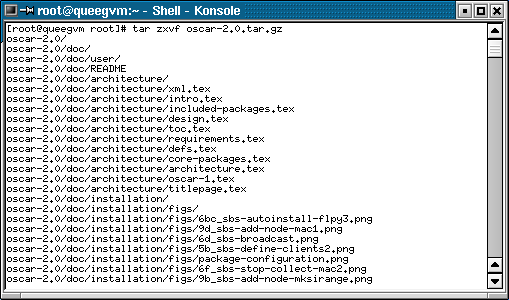
\includegraphics[scale=\imgscale]{figs/0c_sbs-unpack}}
    \caption{Unpacking OSCAR.}
    \label{fig:sbs-unpacking-oscar}
  \end{center}
\end{figure}

%TODO
%TJN: NEW need new capture
\begin{figure}[!ht]
  \begin{center}
    \centerline{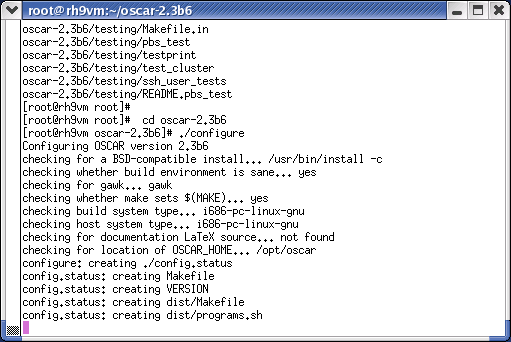
\includegraphics[scale=\imgscale]{figs/sbs-configure-install}}
      \vspace{\imgvskip}
	\centerline{
      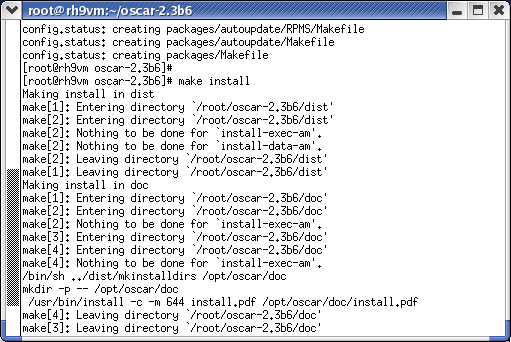
\includegraphics[scale=\imgscale]{figs/sbs-make-install-1}
      \hspace{\imghskip}
      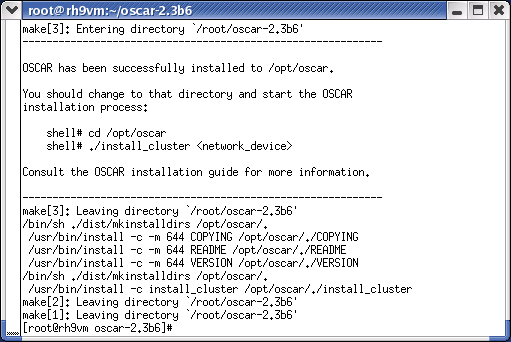
\includegraphics[scale=\imgscale]{figs/sbs-make-install-2}
      }
    \caption{Configure \& Install the OSCAR Toolkit.}
    \label{fig:sbs-configure-install}
  \end{center}
\end{figure}

\begin{figure}[!ht]
  \begin{center}
    \centerline{
      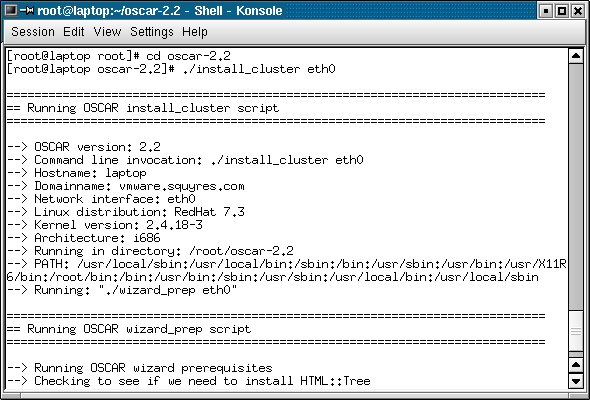
\includegraphics[scale=\imgscale]{figs/1a_sbs-install-oscar}
      \hspace{\imghskip}
      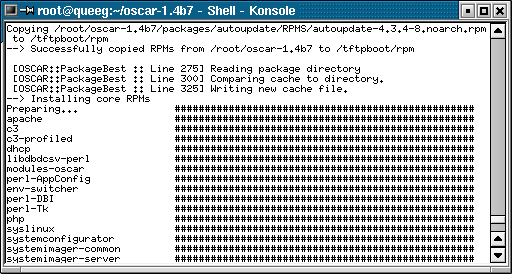
\includegraphics[scale=\imgscale]{figs/1b_sbs-install-oscar2}
      }
    \caption{Running the \cmd{install\_cluster} script.}
    \label{fig:sbs-install-oscar}
  \end{center}
\end{figure}

\begin{figure}[ht!]
  \begin{center}
    \centerline{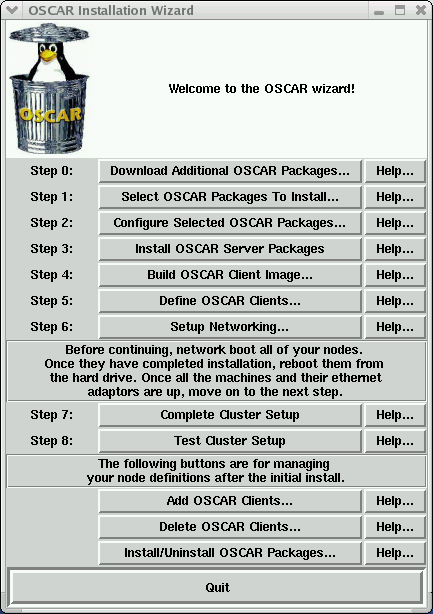
\includegraphics[scale=\imgscale]{figs/2_sbs-oscar-wizard}}
    \caption{The OSCAR Installation Wizard.}
    \label{fig:sbs-install-wizard}
  \end{center}
\end{figure}

%------------------------------------------------------------------
% Select OSCAR packages to download w/ OPD/OPDer
%------------------------------------------------------------------

%TJN: NEW need new capture
\subsection{Download Additional OSCAR Packages...}

An optional step.  See details in Section~\ref{det:opd},
page~\pageref{det:opd}.

\begin{figure}[ht!]
  \begin{center}
    \centerline{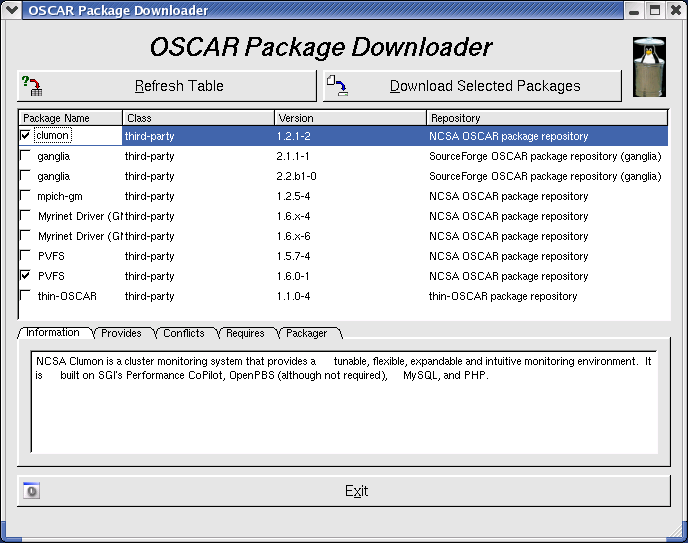
\includegraphics[scale=\imgscale]{figs/sbs-download-packages}}
    \caption[Downloading additional OSCAR packages.]{Selecting additional 
	OSCAR packages to download using OPD/OPDer.}
    \label{fig:sbs-download-packages}
  \end{center}
\end{figure}

\begin{figure}[ht!]
  \begin{center}
    \centerline{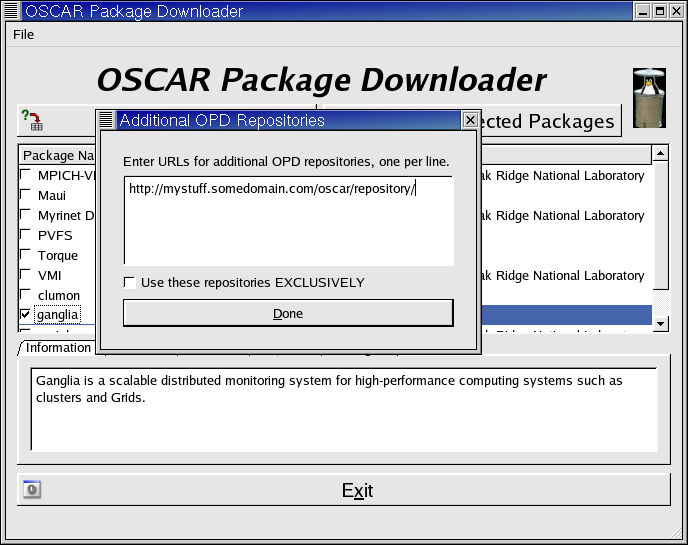
\includegraphics[scale=\imgscale]{figs/sbs-opder-alt-repository}}
    \caption[Adding additional OPD Repositories.]{Adding Additional OPD
        Repositories.}
    \label{fig:sbs-opder-alt-repository}
  \end{center}
\end{figure}

%------------------------------------------------------------------
% Select OSCAR packages to install
%------------------------------------------------------------------

\subsection{Select OSCAR Packages to Install}

An optional step.  See details in Section~\ref{det:select-packages},
page~\pageref{det:select-packages}.

\begin{figure}[ht!]
  \begin{center}
    \centerline{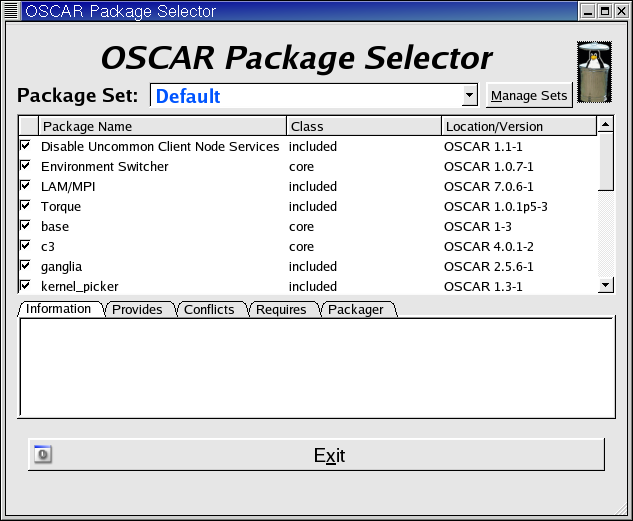
\includegraphics[scale=\imgscale]{figs/package-selection}}
    \caption[Selecting which OSCAR packages to install.]{Selecting
      which OSCAR packages to install.}  
    \label{fig:sbs-package-selection}
  \end{center}
\end{figure}

%------------------------------------------------------------------
% Configure selected OSCAR packages
%------------------------------------------------------------------

\subsection{Configure Selected OSCAR Packages}

An optional step.  See details in
Section~\ref{det:configure-packages},
page~\pageref{det:configure-packages}.

\begin{figure}[ht!]
  \begin{center}
    \centerline{
      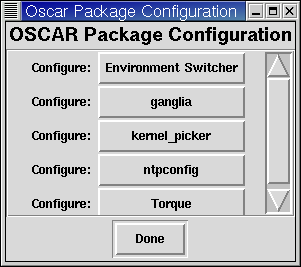
\includegraphics[scale=\imgscale]{figs/package-configuration}
      \hspace{\imghskip}
      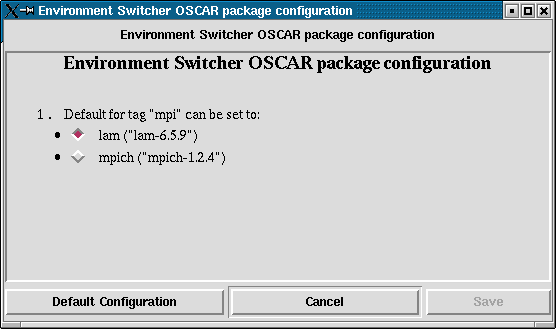
\includegraphics[scale=\imgscale]{figs/package-configuration-switcher}
    }
    \caption{Configuring selected OSCAR packages.  For example, the
      Environment Switcher package has configuration options.}
    \label{fig:sbs-package-configuration}
  \end{center}
\end{figure}

%------------------------------------------------------------------
% Install OSCAR Server Packages
%------------------------------------------------------------------

\subsection{Install OSCAR Server Packages}

This step is used to setup the server for the OSCAR cluster.  See
details in Section~\ref{det:install-server-packages},
page~\pageref{det:install-server-packages}.

\begin{figure}[hb!]
  \begin{center}
    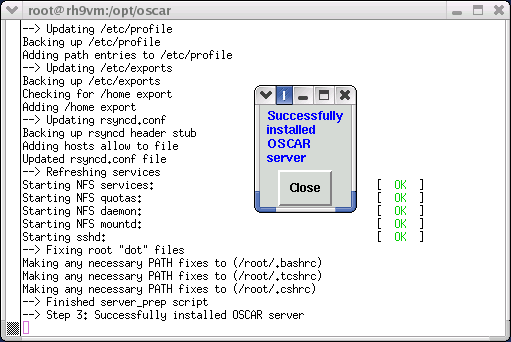
\includegraphics[scale=\imgscale]{figs/install-server-pkgs-done}
    \caption{Successfully installed the OSCAR server packages.}
    \label{fig:sbs-install-wizard-s1}
  \end{center}
\end{figure}


%------------------------------------------------------------------
% Build OSCAR Client Image
%------------------------------------------------------------------

\subsection{Build OSCAR Client Image}

This step builds a disk image for the clients to download and install
onto their local disks.  See the details in
Section~\ref{det:build-client-image},
page~\pageref{det:build-client-image}.

\begin{figure}[!ht]
  \begin{center}
    \centerline{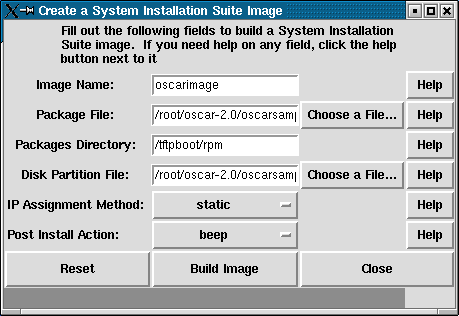
\includegraphics[scale=\imgscale]{figs/4a_sbs-build-image1}}
    \vspace{\imgvskip}
    \centerline{
      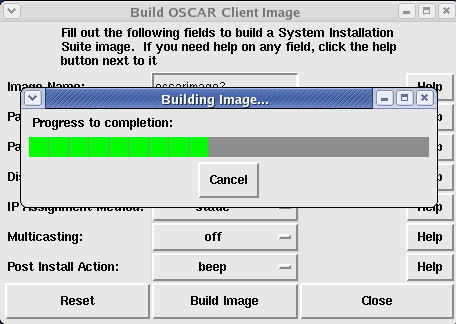
\includegraphics[scale=\imgscale]{figs/4a_sbs-build-image2}
      \hspace{\imghskip}
      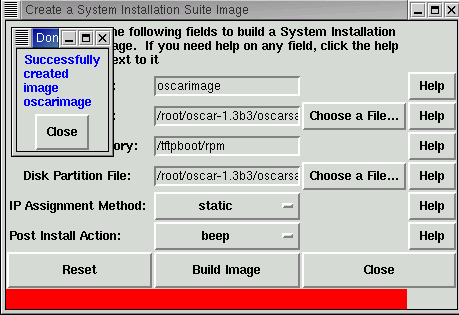
\includegraphics[scale=\imgscale]{figs/4c_sbs-build-image3}
      }
    \caption{Building the OSCAR client image.}
    \label{fig:sbs-build-image}
  \end{center}
\end{figure}


%------------------------------------------------------------------
% Define OSCAR Clients
%------------------------------------------------------------------

\clearpage
\subsection{Define OSCAR Clients}

Step 3 is used to specify how many clients there will be, and what
their TCP/IP characteristics will be.  See the details in
Section~\ref{det:define-clients}, page~\pageref{det:define-clients}.
 
\begin{figure}[ht!]
  \begin{center}
    \centerline{
      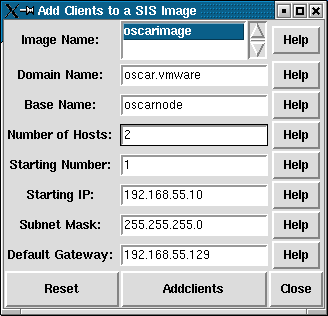
\includegraphics[scale=\imgscale]{figs/5a_sbs-define-clients1}
      \hspace{\imghskip}
      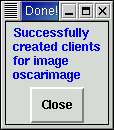
\includegraphics[scale=\imgscale]{figs/5b_sbs-define-clients2}
      }
    \caption{Defining the OSCAR clients.}
    \label{fig:sbs-define-clients}
  \end{center}
\end{figure}


%------------------------------------------------------------------
% Setup Networking
%------------------------------------------------------------------

\subsection{Setup Networking}

This step is used to collect the MAC addresses of the clients, and
then download the disk images to the clients.  See the details in
Section~\ref{det:setup-networking},
page~\pageref{det:setup-networking}.

\begin{figure}[!ht]
  \begin{center}
    \centerline{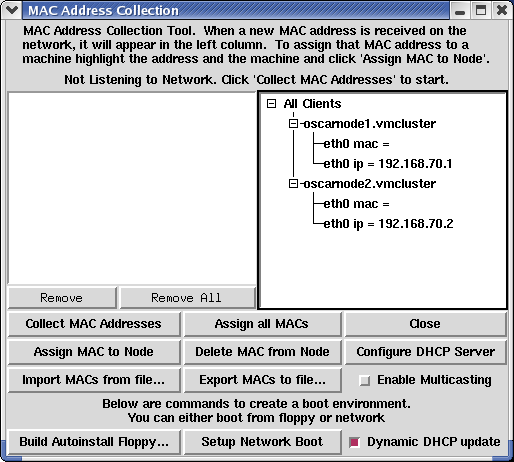
\includegraphics[scale=\imgscale]{figs/6a_sbs-collect-mac1}}
    \caption{Setup networking: initial window.}
    \label{fig:sbs-setup-network1}
  \end{center}
\end{figure}

%-------
% Show how to create the boot CD
%-------

\begin{figure}[!ht]
  \begin{center}
    \centerline{
      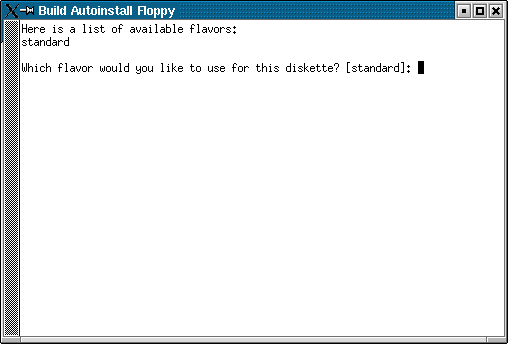
\includegraphics[scale=\imgscale]{figs/6ba_sbs-autoinstall-flpy1}
      \hspace{\imghskip}
      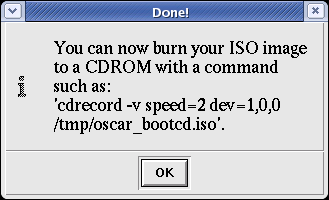
\includegraphics[scale=\imgscale]{figs/6ba_sbs-autoinstall-flpy2}
      }
    \caption{Setup networking: building an autoinstall CD.}
    \label{fig:sbs-autoinstall-flpy1}
  \end{center}
\end{figure}

%-------
% Booting the client
%-------

\begin{figure}[!ht]
  \begin{center}
    \centerline{
      \framebox{
        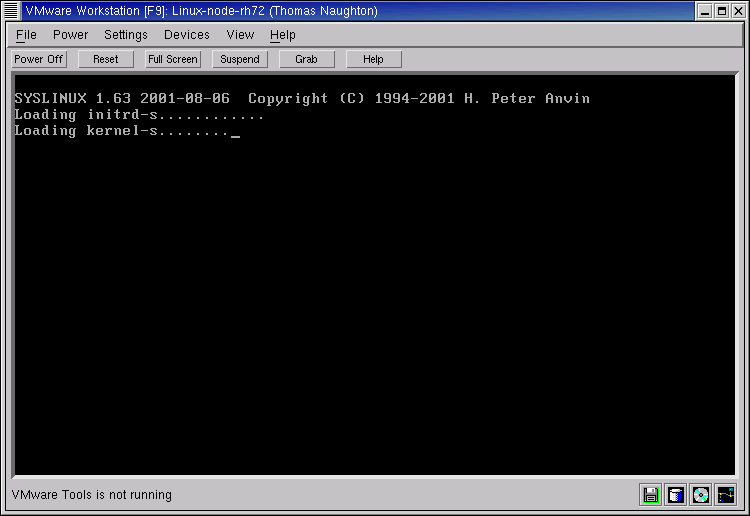
\includegraphics[scale=\imgscale]{figs/6c_sbs-client-boot1}
        }
      }
    \caption{Setup networking: booting the client.}
    \label{fig:sbs-collect-boot1}
  \end{center}
\end{figure}

\begin{figure}[!ht]
  \begin{center}
    \centerline{
      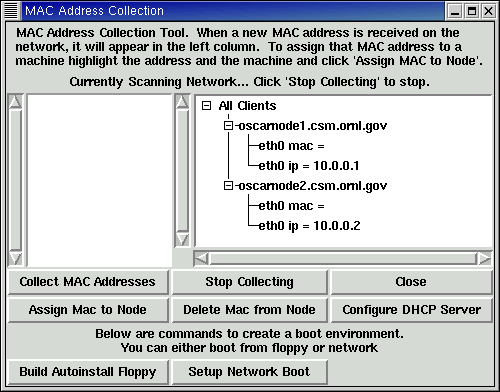
\includegraphics[scale=\imgscale]{figs/6ca_sbs-client-boot1}}
    \caption{Setup networking: scan for booting client (DHCP request).}
    \label{fig:sbs-client-boot2}
  \end{center}
\end{figure}

\begin{figure}[!ht]
  \begin{center}
    \centerline{
      \framebox{
        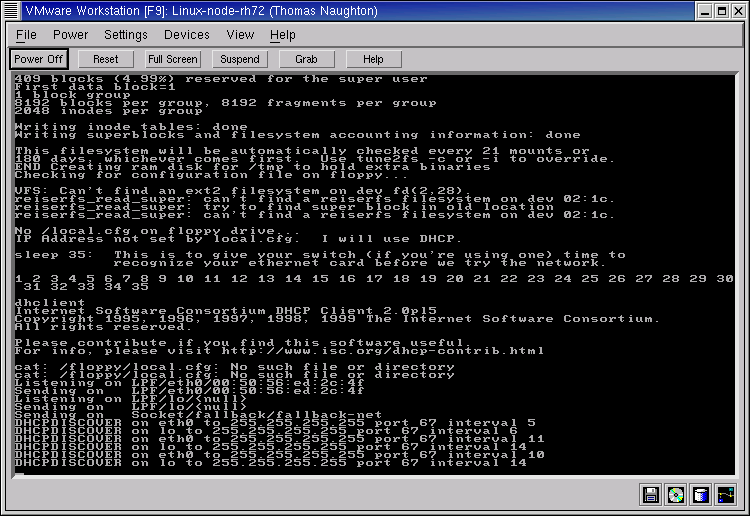
\includegraphics[scale=\imgscale]{figs/6d_sbs-broadcast}
        }
      }
    \caption{Setup networking: client is broadcasting, allows capture
      of MAC address.}
    \label{fig:sbs-collect-broadcast} 
  \end{center}
\end{figure}

\begin{figure}[!ht]
  \begin{center}
    \centerline{
      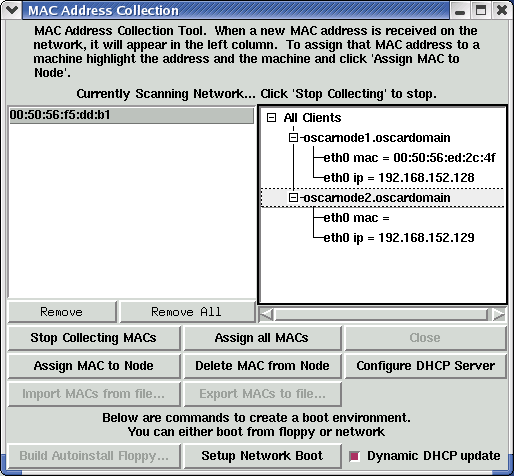
\includegraphics[scale=\imgscale]{figs/6e_sbs-found-mac}
      \hspace{\imghskip}
      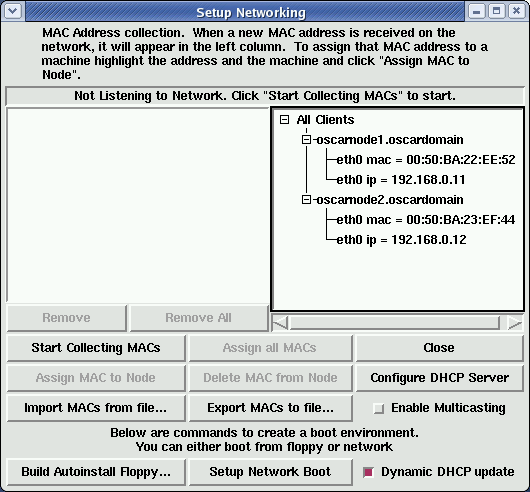
\includegraphics[scale=\imgscale]{figs/6f_sbs-stop-collect-mac2}
    }
    \caption[Setup networking: Assigning MACs to IPs]{Setup
      networking: Scanning network, found first MAC address, then
      later assigned all MAC addresses.}
    \label{fig:sbs-setup-network2}
  \end{center}
\end{figure}

%-------
% SystemImager Monitor
%-------

\begin{figure}[htbp]
  \begin{center}
    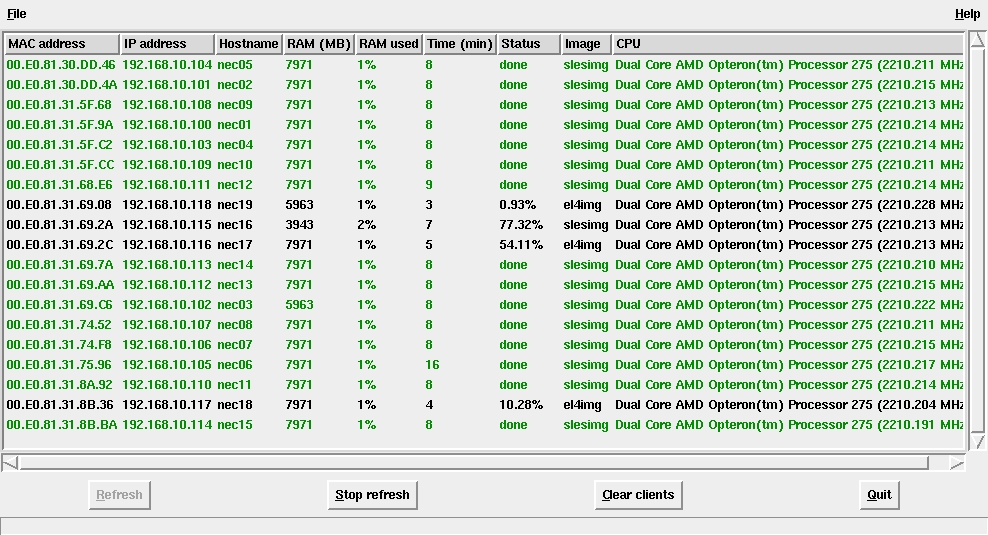
\includegraphics[scale=\imgscale]{figs/si_monitortk}
    \caption{Optional Cluster Deployment Monitor}
    \label{fig:sbs-si-monitortk}
  \end{center}
\end{figure}

%-------
% Client downloading and installing the image
%-------

\begin{figure}[!ht]
  \begin{center}
    \centerline{
      \framebox{
        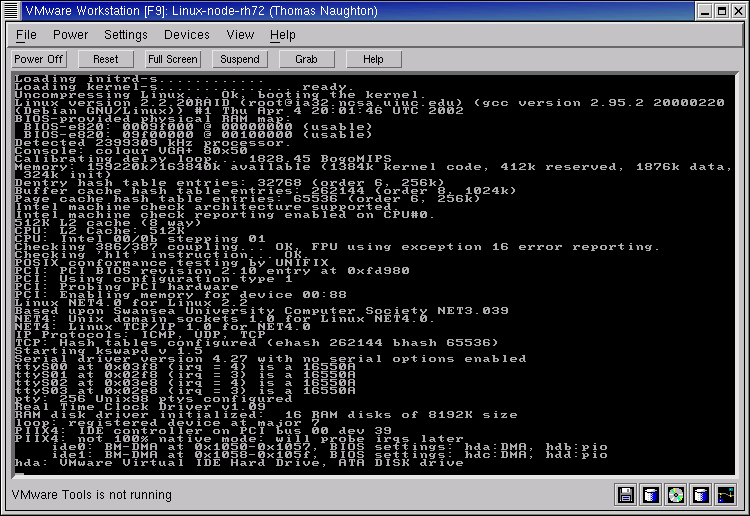
\includegraphics[scale=\imgscale]{figs/6h_sbs-client-boot}
        }
      }
    \caption{Booting the client a second time to download the image.}
    \label{fig:sbs-install-boot}
  \end{center}
\end{figure}

\begin{figure}[!ht]
  \begin{center}
    \centerline{
      \framebox{
        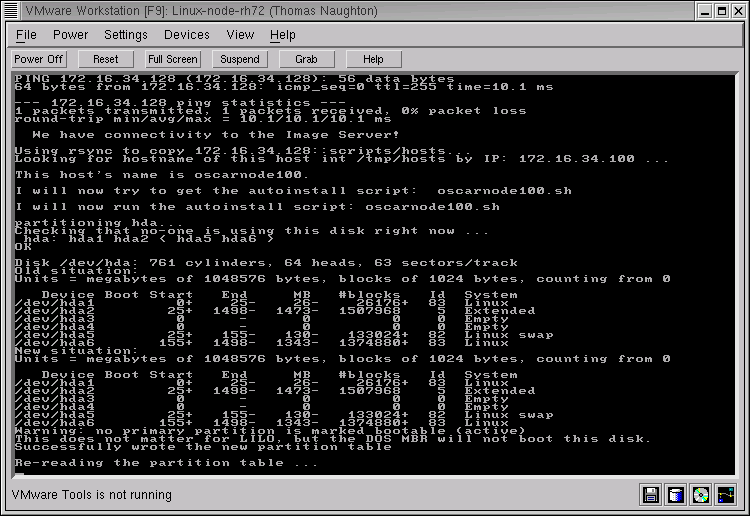
\includegraphics[scale=\imgscale]{figs/6i_sbs-client-diskpar}
        }
      }
    \caption{Client partitioning disk, setting up the disk tables, and
      starting to download the image.}
    \label{fig:sbs-install-diskpar}
  \end{center}
\end{figure}
  
\begin{figure}[!ht]
  \begin{center}
    \centerline{
      \framebox{
        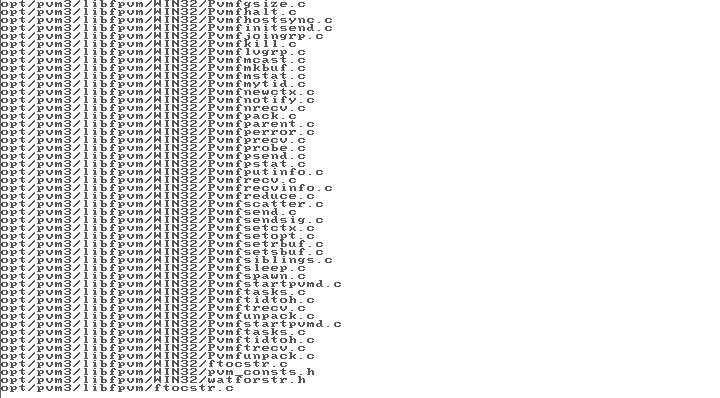
\includegraphics[scale=\imgscale]{figs/6j_sbs-client-rsync}
        }
      }
    \caption{Client downloading and installing the image.}
    \label{fig:sbs-install-rsync}
  \end{center}
\end{figure}

\begin{figure}[!ht]
  \begin{center}
    \centerline{
      \framebox{
        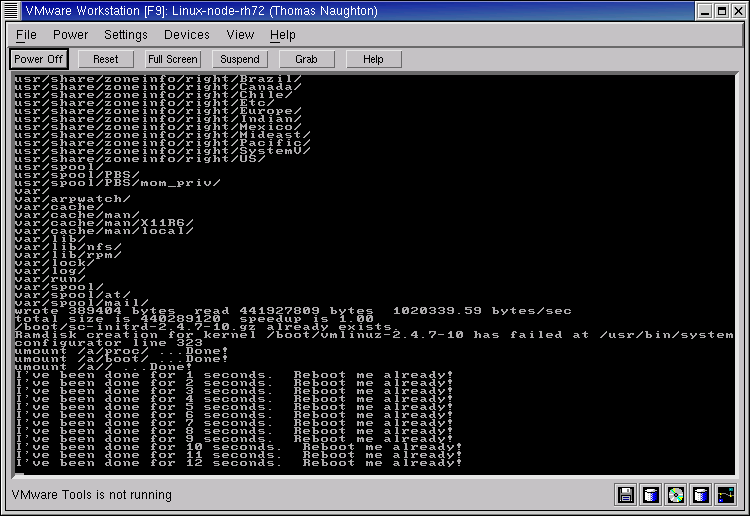
\includegraphics[scale=\imgscale]{figs/6k_sbs-rebootme}
        }
      }
    \caption{A client has finished the install and is asking to be
      rebooted.} 
    \label{fig:sbs-install-finish}
  \end{center}
\end{figure}


%------------------------------------------------------------------
% Complete Cluster Setup
%------------------------------------------------------------------

\clearpage
\subsection{Step 5: Complete Cluster Setup} 

This step is used to unify the server and client installations into a
single cluster.  See the details in
Section~\ref{det:complete-cluster-setup},
page~\pageref{det:complete-cluster-setup}.

\begin{figure}[!ht]
   \begin{center}
     \centerline{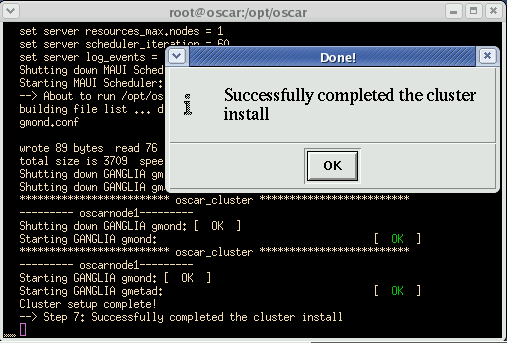
\includegraphics[scale=\imgscale]{figs/7_sbs-complete-cluster-setup}}
     \caption{Complete Cluster Setup.}
     \label{fig:sbs-install-wizard-s5}
   \end{center}
 \end{figure}


%------------------------------------------------------------------
% Test Cluster Setup
%------------------------------------------------------------------

\subsection{Test Cluster Setup}

This step is used to test the cluster setup.  It can either be run
from within the wizard, or, as shown here, from manually launching a
shell script at a \user{root} command prompt.  See the details in
Section~\ref{det:test-cluster}, page~\pageref{det:test-cluster}.

\begin{figure}[!ht]
  \begin{center}
    \centerline{
      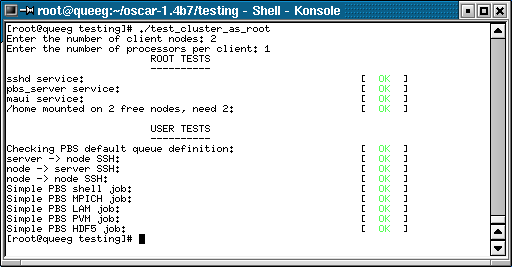
\includegraphics[scale=\imgscale]{figs/8_test-cluster-complete}
      }
    \caption{Test the cluster.}
    \label{fig:sbs-setup-test}
  \end{center}
\end{figure}


%-----------------------------------------------------------------
% Delete Node Button
%-----------------------------------------------------------------

\subsection{Delete Node Button}
\label{app:sbs-delete-node}

The Delete Node button can be used to delete clients from an OSCAR
cluster.  Note that this button only deletes OSCAR's knowledge of the
clients -- what physically happens to that client is not OSCAR's
concern.  This example shows deleting one of the clients setup in the
previous sections -- \hostname{oscarnode2}.  The next section
(Section~\ref{app:sbs-add-node}) will show adding it back.  See the
details on deleting clients in Section~\ref{det:deleting-clients},
page~\pageref{det:deleting-clients}.

\begin{figure}[!ht]
  \begin{center}
    \centerline{
      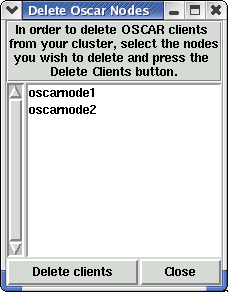
\includegraphics[scale=\imgscale]{figs/10a_sbs-del-node}
      \hspace{\imghskip}
      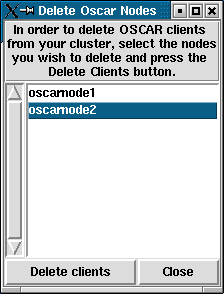
\includegraphics[scale=\imgscale]{figs/10b_sbs-del-node-partA}
      \hspace{\imghskip}
      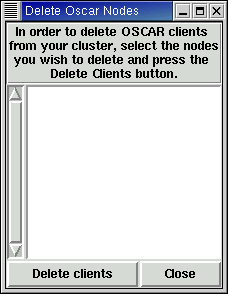
\includegraphics[scale=\imgscale]{figs/10b_sbs-del-node-partB}
      }
    \caption[Delete OSCAR Clients.]{Delete OSCAR clients.  First image
    is the initial window, second image is with a client selected, and
    third image is when the action has completed.}
    \label{fig:sbs-del-node1}
  \end{center}
\end{figure}


%------------------------------------------------------------------
% Add Node Button
%------------------------------------------------------------------

\subsection{Add Node Button}
\label{app:sbs-add-node}

The Add Node button will add clients into an existing OSCAR cluster.
In this example, we will add back \hostname{oscarnode2} into the
cluster.  See the details of adding a client in
Section~\ref{det:adding-clients}, page~\pageref{det:adding-clients}.

\begin{figure}[!ht]
  \begin{center}
    \centerline{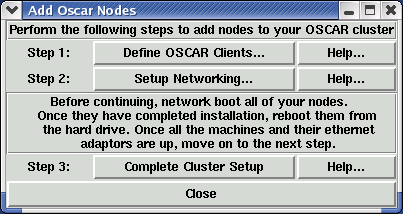
\includegraphics[scale=\imgscale]{figs/9a_sbs-add-node}}
    \caption{Add OSCAR Clients.}
    \label{fig:sbs-add-node1}
  \end{center}
\end{figure}

\begin{figure}[!htb]
  \begin{center}
    \centerline{
      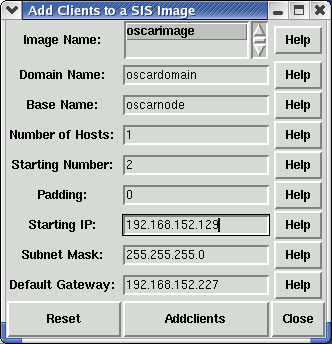
\includegraphics[scale=\imgscale]{figs/9b_sbs-add-node-mksirange}
      \hspace{\imghskip}
      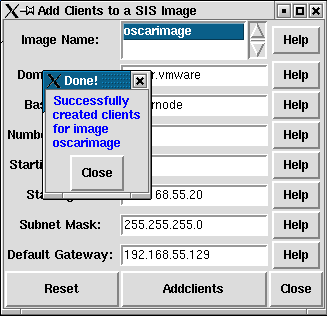
\includegraphics[scale=\imgscale]{figs/9c_sbs-add-node-success}
      }
    \caption{Add node / defining the clients.}
    \label{fig:sbs-add-node1-define-clients}
  \end{center}
\end{figure}

\begin{figure}[!t]
  \begin{center}
    \centerline{
      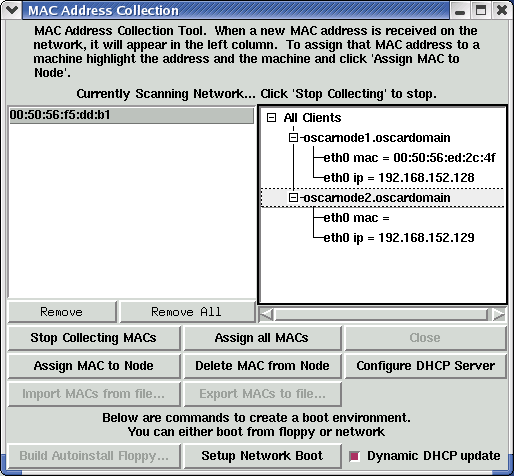
\includegraphics[scale=\imgscale]{figs/6e_sbs-found-mac}
      \hspace{\imghskip}
      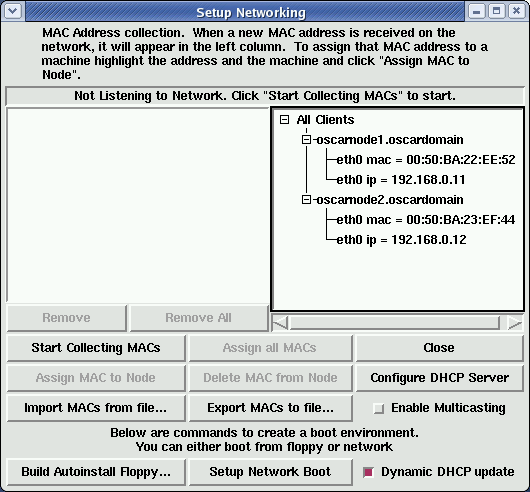
\includegraphics[scale=\imgscale]{figs/6f_sbs-stop-collect-mac2}
%      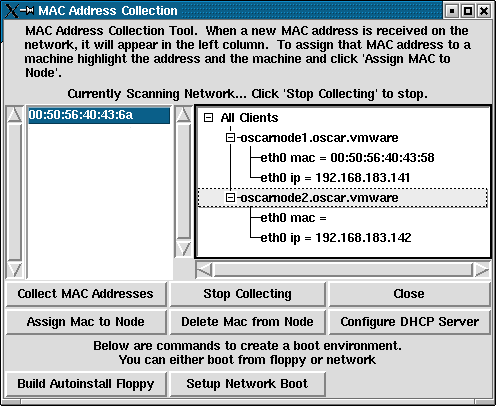
\includegraphics[scale=\imgscale]{figs/9d_sbs-add-node-mac1}
%      \hspace{\imghskip}
%      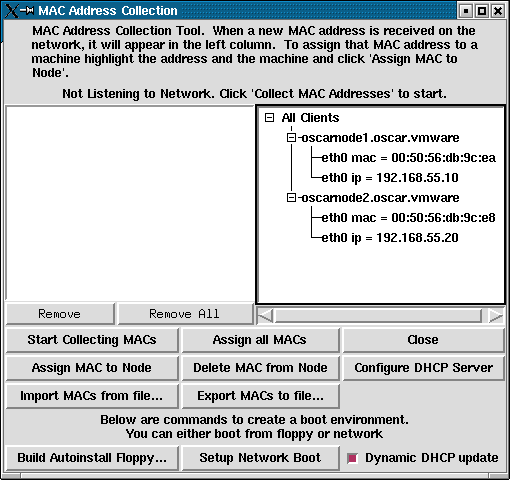
\includegraphics[scale=\imgscale]{figs/9e_sbs-add-node-mac2}
      }
    \caption{Add node / setup networking.}
    \label{fig:sbs-add-node1-setup-network}
  \end{center}
\end{figure}

\begin{figure}[!b]
  \begin{center}
    \centerline{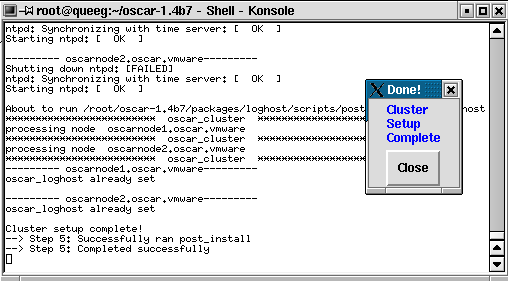
\includegraphics[scale=\imgscale]{figs/9f_sbs-add-node-complete}}
    \caption{Add node / complete cluster setup.}
    \label{fig:sbs-add-node1-cluster-setup}
  \end{center}
\end{figure}

%------------------------------------------------------------------
% Install/Uninstall OSCAR Packages
%------------------------------------------------------------------

\subsection{Install/Uninstall OSCAR Packages}

The Install/Uninstall OSCAR Packages button will let you add/remove packages from
and an OSCAR cluster after the initial installation.  See the details and more
in-depth look at the underlying concepts of this new feature in
Section~\ref{det:install-uninstall-packages}, page~\pageref{det:install-uninstall-packages}.

\begin{figure}[ht!]
  \begin{center}
    \centerline{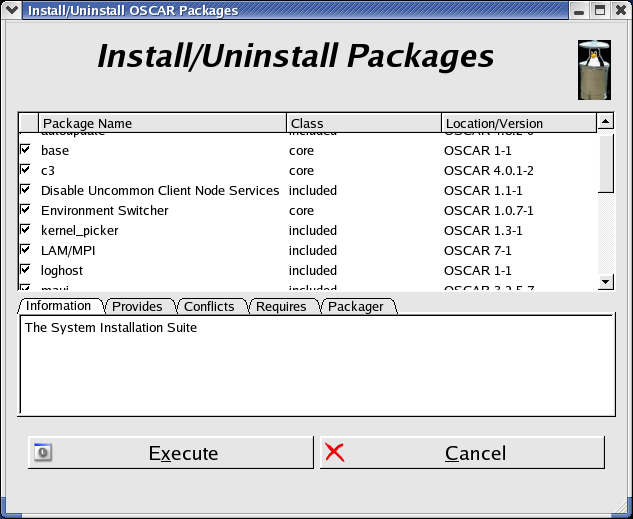
\includegraphics[scale=\imgscale]{figs/sbs-pkgInUn-selector}}
    \caption[Install/Uninstall OSCAR Packages.]{Install/Uninstall packages from an existing
        OSCAR cluster.}
    \label{fig:sbs-pkgInUn-selector}
  \end{center}
\end{figure}

\begin{figure}[ht!]
  \begin{center}
    \centerline{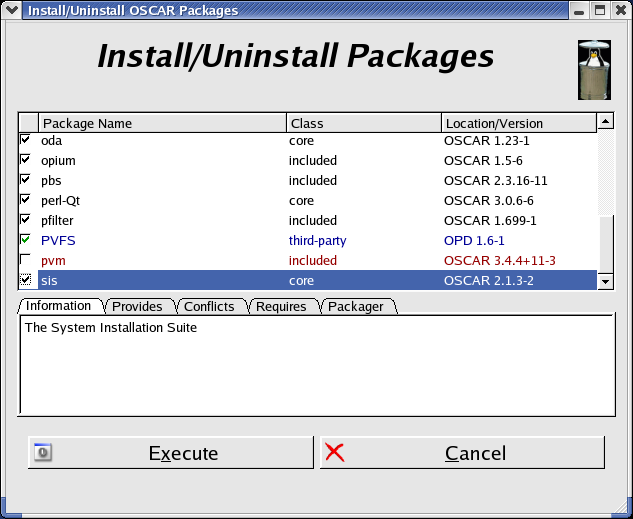
\includegraphics[scale=\imgscale]{figs/sbs-pkgInUn-selector-example-colors}}
    \caption[Install/Uninstall OSCAR Package selector sample colors.]{Individual OSCAR packages
        are color-coded to show their current installation state.}
    \label{fig:sbs-pkgInUn-selector-example-colors}
  \end{center}
\end{figure}

% LocalWords:  tex Exp sbs
